\chapter{Getting Started}\label{ch:K01_Getting_Started}
\section{Installation von Python und VS Code}
Die aktuellen Installationsanleitungen für Windows und MacOS finden Sie auf unserer GitHub-Pages-Website:

\begin{center}
    \url{https://cyrilblum.github.io/LeeTeX/vscode-python-setup.html}
\end{center}

Dort sind alle Schritte inklusive Abbildungen laufend aktuell dokumentiert.

\section{Erstes Python-Programm schreiben und ausführen}
Jetzt schreiben wir unser erstes Python-Programm! Dieses besteht aus nur einer einzigen Zeile und lautet:

\lstinputlisting[language=Python,caption=\texttt{hello\_world.py},label=listing:hello_world]{Grundlagen_Info/00_Programmieren/Skript/Code/K01_Getting_Started/hello_world.py}

Die kleine Ziffer \texttt{1} ist die Zeilennummer (diese wird vom Code-Editor automatisch gesetzt). Wir führen nun das Programm aus (\enquote{lassen das Programm laufen}), indem wir (oben rechts) auf den \emoji{play-button}-Knopf klicken. Bei uns sieht die Situation aus wie in \cref{fig:runHelloWorld}.
\begin{figure}[H]
    \centering
    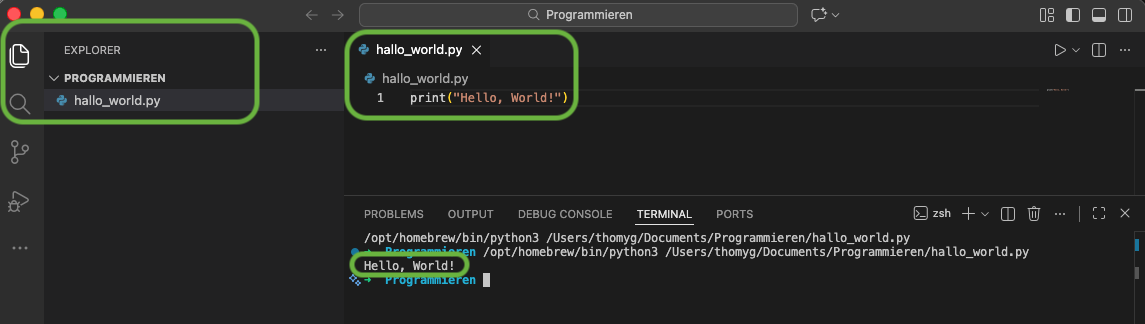
\includegraphics[width=0.9\textwidth]{Grundlagen_Info/00_Programmieren/Skript/Figures/VSCode_RunHelloWorld.png}
    \caption{Python-Programm \texttt{hello\_world.py} in VS Code ausführen.}
    \label{fig:runHelloWorld}
\end{figure}
\cref{listing:hello_world}, macht nichts weiter, als den Text
\begin{center}
    \texttt{Hello, World!}
\end{center}
im Terminal (Englisch: \texttt{terminal}) auszugeben\footnote{\url{https://de.wikipedia.org/wiki/Hallo-Welt-Programm}}.